\documentclass[main.tex]{subfiles} 
\begin{document}

\section*{Teoretisk bakgrunn}
Gjennom underveisvurderingen følges elevenes progresjon
i faget over tid, og læreren får informasjon
om oppnådd kompetanse.

Det er ikke bare den faglige vurderingen som skal evalureres gjennom en skolegang. Ludvigsens utvalget mener
at den sosiale og emosjonelle utviklingen bør også ha større plass i vurderingsgrunnlaget enn det har idag :
\begin{displayquote}
Utvalget fremhever betydningen av et bredt kompetansebegrep,
og at skolen mer systematisk enn
i dag skal støtte elevenes sosiale og emosjonelle
læring og utvikling i fagene. For eksempel skal
elevene utvikle nysgjerrighet, selvregulering og
respekt for andres synspunkter. Sosiale og emosjonelle
kompetanser er ikke vektlagt systematisk
i dagens læreplaner, og det er derfor en endring
sammenlignet med i dag når dette blir en tydeligere
del av kompetansemålene i fagene. Dette
gir noen utfordringer som må håndteres på en
god måte i bestemmelser for vurdering og i lærernes
praksis. (NOU 2015: Fremtidens skole)
\end{displayquote}

Et prinsipp bør være at mål for elevenes sosiale
og emosjonelle kompetanse ikke tillegges vekt
i seg selv i den samlede sluttvurderingen, men at
de ses som forutsetninger for den kompetansen
elevene viser i faget.

\begin{figure}[h!]
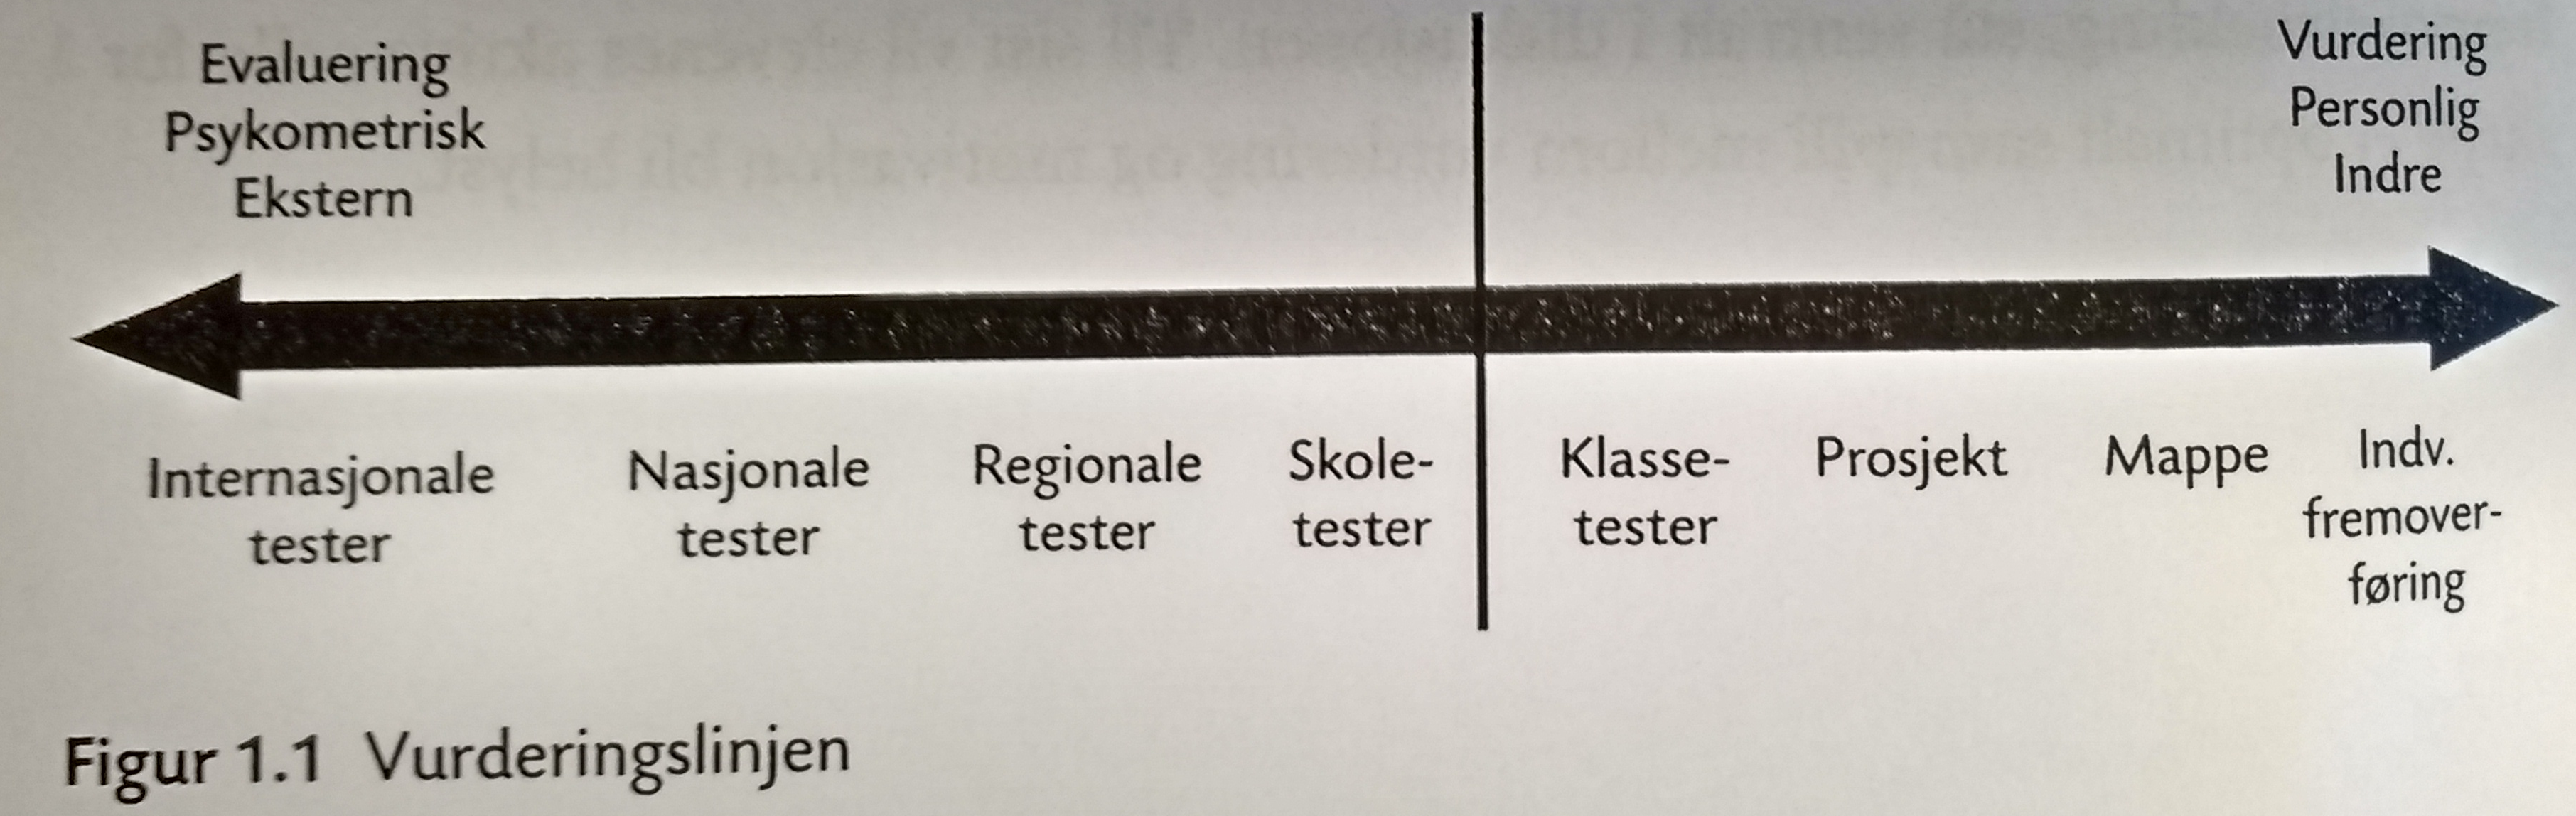
\includegraphics[scale = 0.1]{../figures/vurderingslinjen.png}
%\caption{Oversikt over naturfaglærernes undervisningstilbud til elevene fra PISA+ studie. Kilde: 
%\protect\citeA{odeg10}.}
%\label{fig:odeg10}
\end{figure}

Skriv om : Summativ vs formativ vurdering
\\
\\
I læringsrettet vurdering stilles det strengere krav til lærerers evner som evaluator. Da er det viktig å se på lærerens læringssyn. Her er to eksempeler på forskjellige læringssyn :
\\
\\
\textbf{Læring som overføring av kunnskap}
\\
I behavioristisk læringsteori foregår læring ved overføring av kunnskap, uavhengig av relasjonen mellom lærer og elev. Elev blir anskuet som et tomt kar, som det er lærerens jobb å fylle
med kunnsakp. I et slikt læringssyn er vurdering i seg selv relativt ukomplisert, siden da gjelder det å formulere sine tilbakemeldinger på en så presis og elevtilpasset måte som mulig.
Derimot forventes det da at eleven tar til seg tilbakemeldingene og bruker den til å rette seg etter.
\\
\\
\textbf{Læring som en relasjonell prosess}
\\
Sett fra den relasjonelle perspektivet består det i å veilede elevene i den nærmeste utviklingssonen.
Den \emph{nærmeste utviklingssonen} beskriver en sone som ligger i mellom en elevs kognitive 
ferdigheter, dvs. hva de kan oppnå selvstendig uten hjelp, og elevens potensielle utvikling, dvs. 
hva en elev kan få til eller forstå gjennom veiledning (\citeNP[s. 125]{bta98}; \citeNP[s. 75]{rogs13}). 
Brukt av ``scaffolding'' eller stillasbygging (\citeNP{bta98}) er da viktig for å knytte fagbegreper og teori til elevenes 
forkunnskaper.
\\
\\
Jeg vil komme tilbake til disse læringssyn når jeg evaluerer min egen praksis gjennom FoU arbeidet.
\end{document}
